\chapter{Simulation}
	To test the performance of the guidance system, it is implemented in matlab/simulink. A number of
	scenarios are used to test how it performes in various conditions.

	The proposed system are greatly simplyfied and there are a number of situations that it will not work
	well. This situations are also threated and discussed in the next chapter. 
	

\section{Matlab}
	The mathematical model of the \textit{HUGIN 1000} AUV are implemented in simulink using the
	\textit{GNC} toolbox available from \textit{www.marinecontrol.org} with slight modifications to the
	6DOF model.

	The Camera output simulator were programmed in matlab. It inputs the position of the AUV and
	transposes it to body coordinates to calculate the field of view of the camera. The camera are based
	on the pinhole camera model with unity focus distance, and a view angle of about 45 degrees. The
	program then calculates the field of view of the camera and checks if there are any part of the
	pipeline inside the field of view. The output of the camera are three points taken out at the top, the
	middle and the bottom of the field of view.

	A sonar which determines the altitude are implemented using a look-up table with a predefined bottom
	profile.

	The descision logic is implemented as a state machine with three states, and gives out the 
	desired heading dependent on what state the system is in.

	The filter was created using a m-file and global variables for the filter parameters. The filter
	parameters are as follows:
	\begin{equation}
		P_0 = \left [ \begin{matrix}
				10 & 0 & 0 & 0 \\
				0 & 10 & 0 & 0 \\
				0 & 0 & 0.1 & 0 \\
				0 & 0 & 0 & 0.1
				\end{matrix} \right] \quad
		W = 0.1 \mathbf{I}_{2x2} \quad Q = 10 \mathbf{I}_{2x2} 
	\end{equation}

	The final simulink diagram are shown in figure \ref{fig:ch3_simulink}.
	\begin{figure}[htbp]
		\centering
		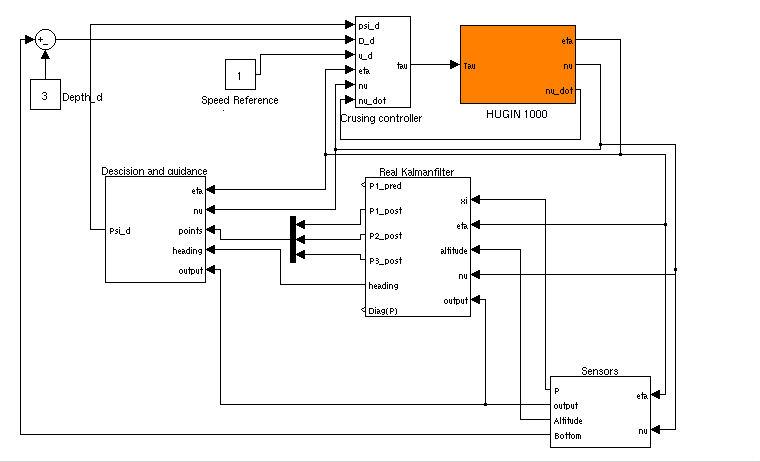
\includegraphics[width=\textwidth]{pics/simulink}
		\caption{The Simulink Diagram of the implemented Guidance System}
		\label{fig:ch3_simulink}
	\end{figure}

	

\section{Simulation Scenarios}
	To test the performance of the guidance system some scenarios are proposed.
	\begin{description}
		\item[\textbf{1$^{\mathrm{st}}$ Scenario}.] The pipeline are at the exact location acording 
		to predefined data. Environmental disturbances such as currents are turned off. The pipelien are
		continiously visible for the camera the whole inspection distance. Reference simulation.
		\item[\textbf{2$^{\mathrm{nd}}$ Scenario}.] Exact as over but with environmental forces turned on.
		\item[\textbf{3$^{\mathrm{rd}}$ Scenario}.] The pipeline are at the exact location where 
		it initially was layed. A section is burried, and not visible for the camera. Environmental
		forces are turned on.
		\item[\textbf{4$^{\mathrm{th}}$ Scenario}.] The \'a priori information about the pipeline 
		are offset about 20 meteres to test the ability of the guidance system to search for the pipeline.
	\end{description}


\section{Results}
	Some of the results for the simulations scenarios are given here. But first a test of the low-speed
	assumptions made for the controller design for the AUV. 

	\subsection{Test of the low-speed assumtion}
		In figures \ref{fig:ch3_coriolis_forces} and \ref{fig:ch3_damping_forces} the forces and
		moments created by the Coriolis/centripetal and damping matrices are recorded. In Figure
		\ref{fig:ch3_coriolis_forces} the sway degree of freedom are dominant, and peaking about
		-400N during the turning maneuvers of the AUV. The forces and moments created by the coriolis
		terms are partially counteracted by the damping terms, that also have greated magnitude than
		the coriolis terms.
		\begin{figure}[htbp]
			\centering
			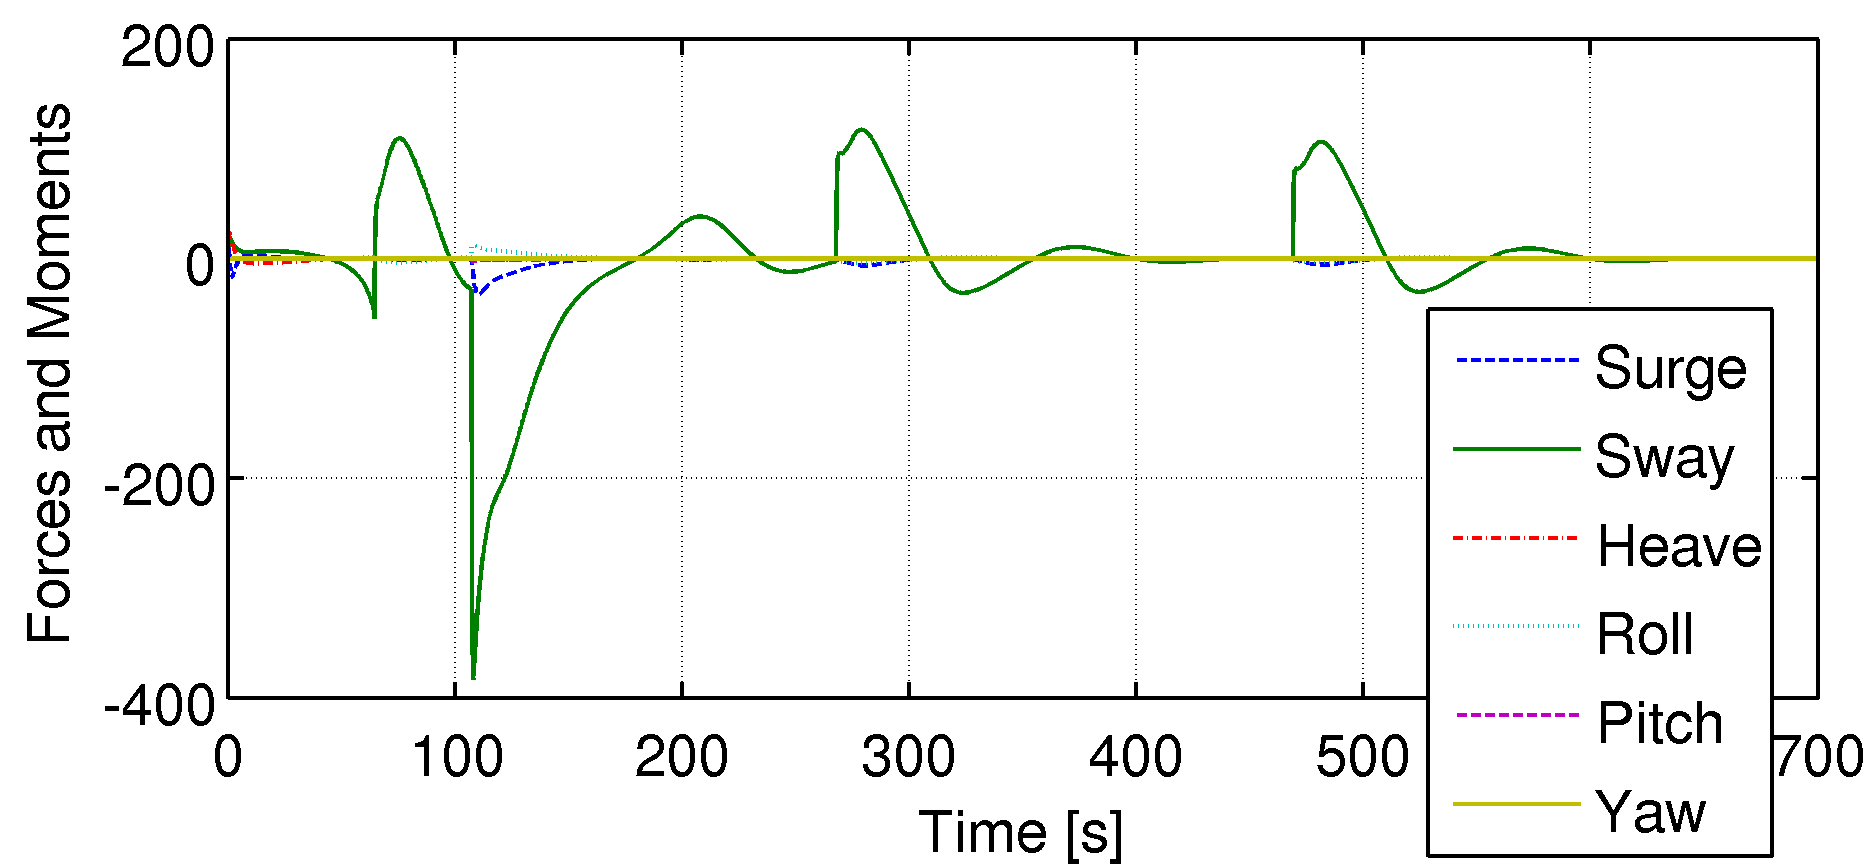
\includegraphics[width=0.7\textwidth]{pics/coriolis_forces}
			\caption{Plot of the Coriolis Forces Associated with the AUV Model}
			\label{fig:ch3_coriolis_forces}
		\end{figure}		
		\begin{figure}[htbp]
			\centering
			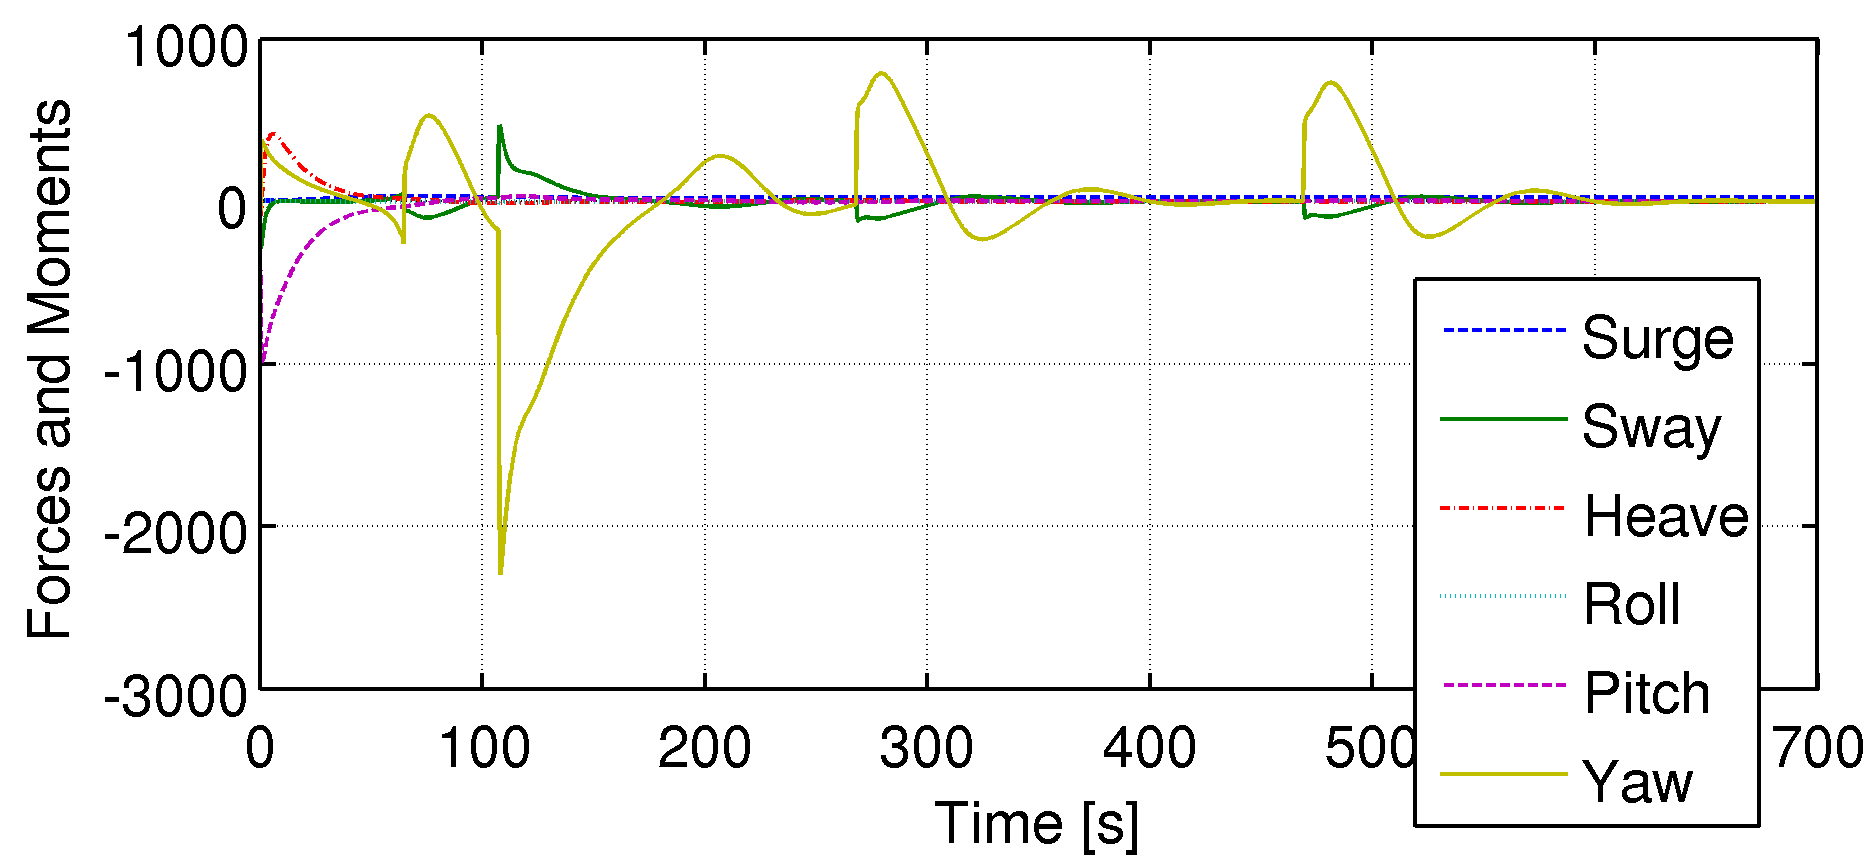
\includegraphics[width=0.7\textwidth]{pics/damping_forces}
			\caption{The Dampering Forces Associated with the AUV when Maneuvering}
			\label{fig:ch3_damping_forces}
		\end{figure}
		This suggests that the coriolis/centripetal forces can be neglected and compensated for as
		model errors in the controller using integral terms.  

	\subsection{1$^{\mathrm{st}}$ Scenario}
		This is mostly a reference test to see how the guidance system performs on the ideal case.
		This can show how sensitive the guidance system are with regard to current disturbances.
		\begin{figure}[htbp]
			\centering
			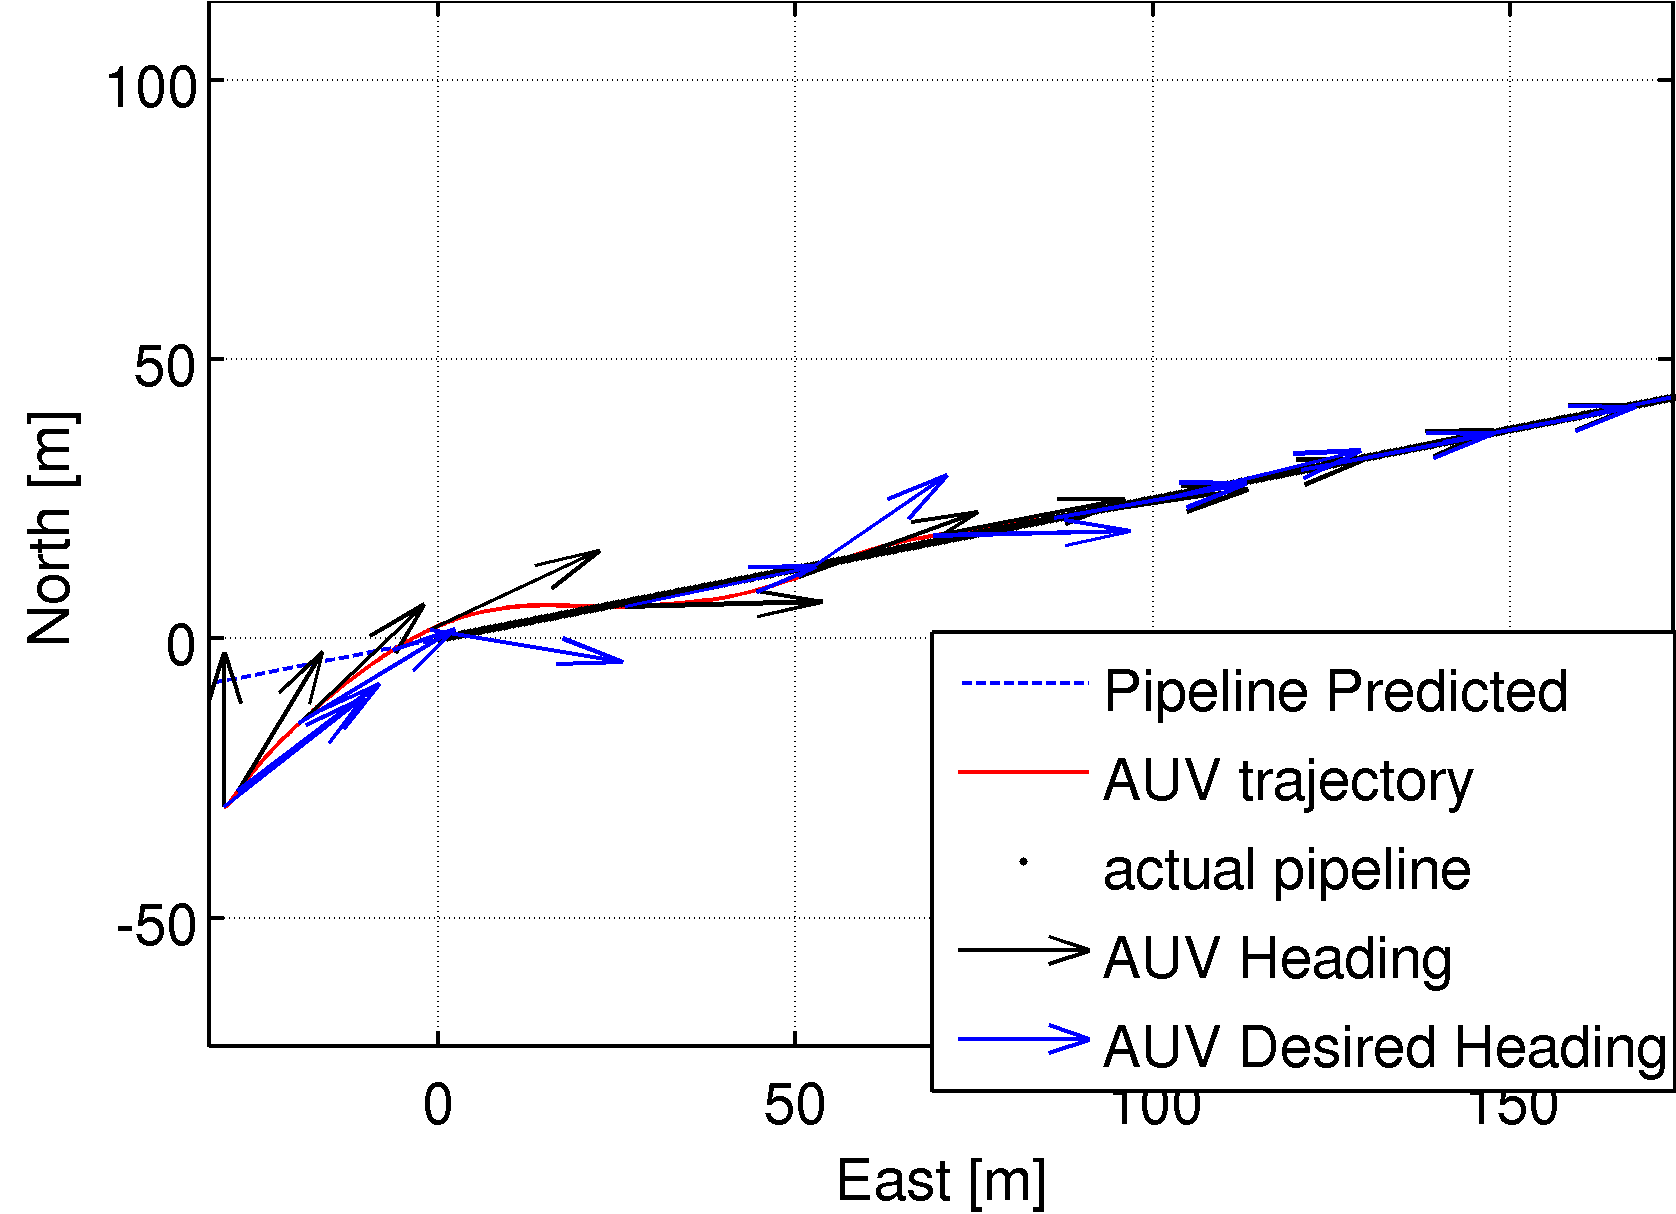
\includegraphics[width=0.7\textwidth]{pics/1st_NE_path}
			\caption{North East path of AUV without Current}
			\label{fig:ch3_1st_NE_path}
		\end{figure}
		\begin{figure}[htbp]
			\centering
			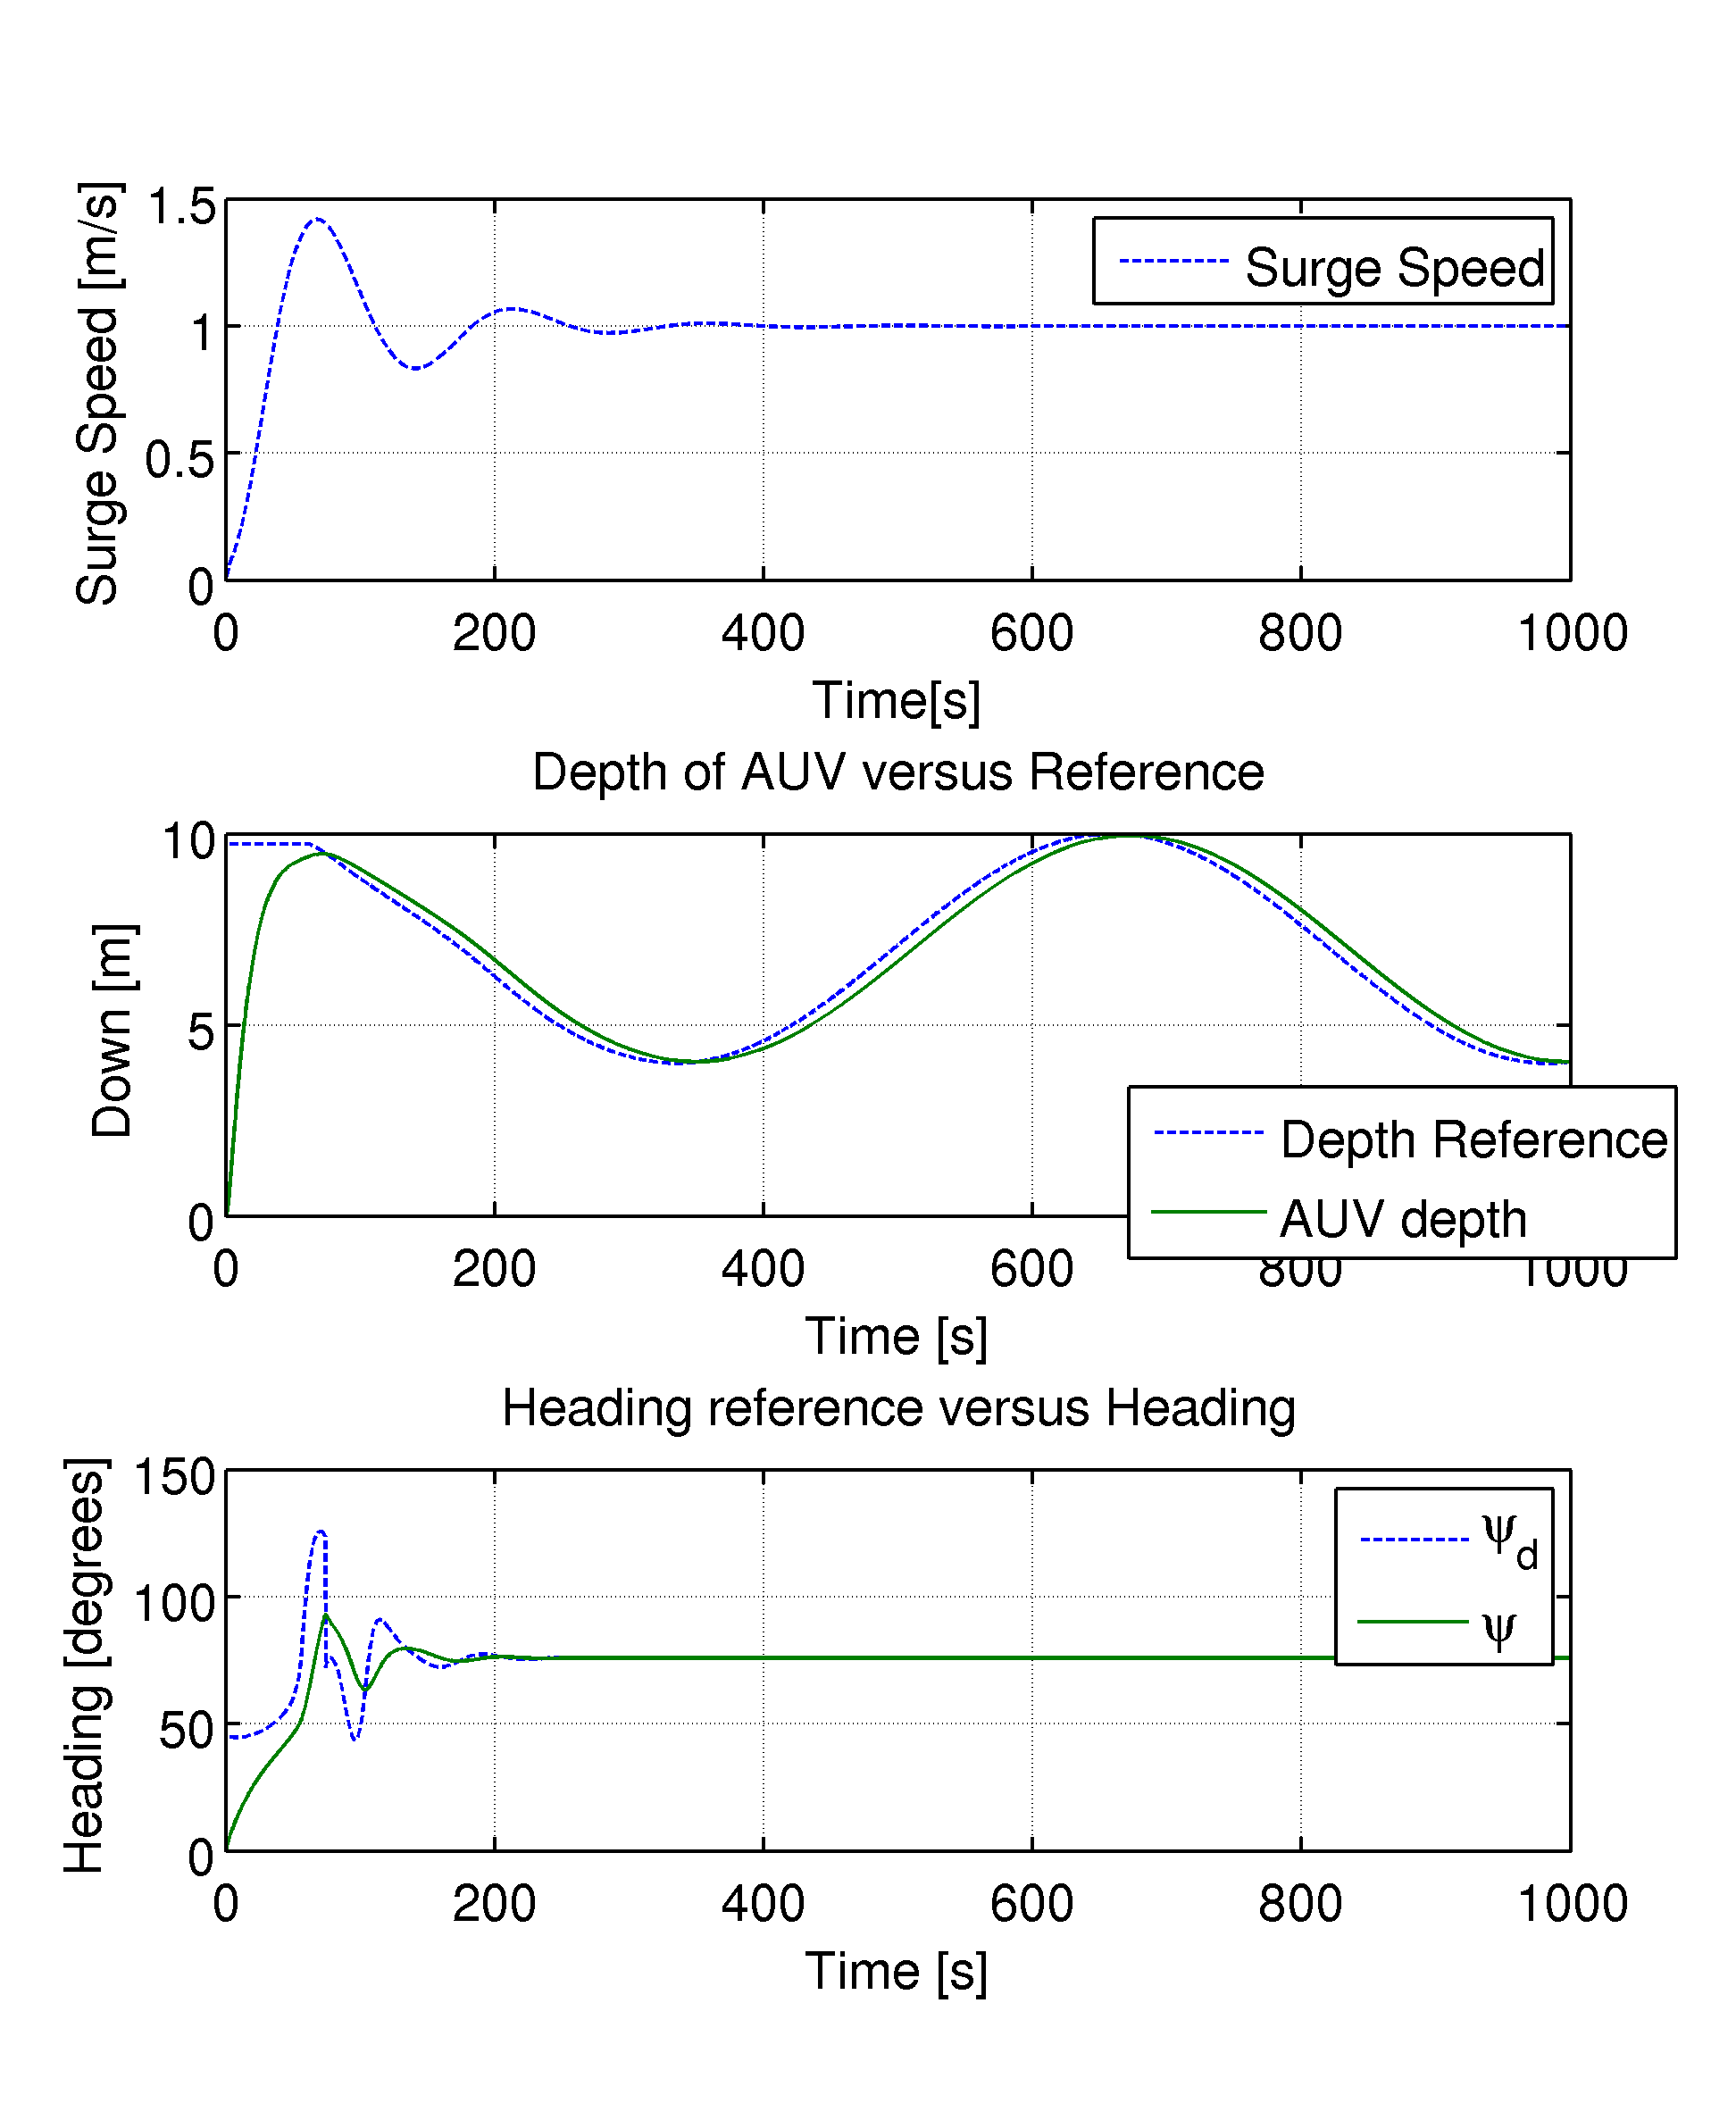
\includegraphics[width=0.75\textwidth]{pics/1st_uDpsi}
			\caption{Surge-, Depth- and Heading- Reference vs. Actual Values}
			\label{fig:ch3_1st_uDpsi}
		\end{figure}
		The result of this test is purly for reference but it might be an idea to notice some things
		about the simulations. 
		
		It can be seen from both Fiugre \ref{fig:ch3_1st_NE_path} and the
		third plot on Figure \ref{fig:ch3_1st_uDpsi} that the heading reference, $\psi_d$ have some
		oscilatory nature. This is because of the relatively low look-ahead distance defined in the
		guidance algorithm. This can be analogus to when driving a car and you fix your gaze on
		the road not very far ahead of the car, and you will get more uneasy driving and not so smooth motion. 

		The depth reference are given by the bottom which are constructed using a look-up table
		created by a sinuosidal plane. The reference are followed pretty well. The delay on the
		action by the controller are created because the \textit{heave} direction are not directley
		controlled, but are relayed through the \textit{pitch} degree of freedom.

	
	\subsection{2$^{\mathrm{nd}}$ Scenario}
	
	
	
	\subsection{3$^{\mathrm{rd}}$ Scenario}
	
	
	
	\subsection{4$^{\mathrm{th}}$ Scenario}

